\subsection{Time series components touched - 14 For packages touched for  each week commit} 
\begin{figure}
  \centering 
  \begin{subfigure}[b] 
{0.45\textwidth}
    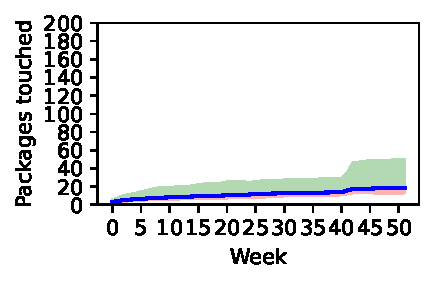
\includegraphics{sections/results/14/packages/time_series_components_touched.packages.all.founders.week_52.pdf}
    \caption{Packages for All founders (n=29, $\mu$=18.62, median=5.0 \& std=16.72)}
    \label{figure.sections/results/14/packages/time_series_components_touched.packages.all.founders.week_52.pdf}
  \end{subfigure}
  \begin{subfigure}[b] 
{0.45\textwidth}
    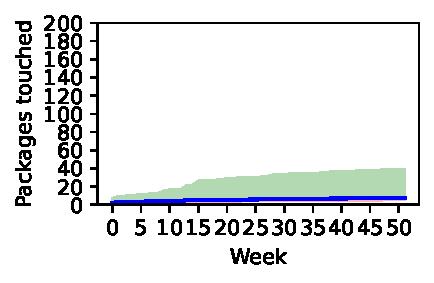
\includegraphics{sections/results/14/packages/time_series_components_touched.packages.all.joiners.week_52.pdf}
    \caption{Packages for All joiners (n=637, $\mu$=7.31, median=2.0 \& std=13.53)}
    \label{figure.sections/results/14/packages/time_series_components_touched.packages.all.joiners.week_52.pdf}
  \end{subfigure}
\newpage 
  \begin{subfigure}[b] 
{0.45\textwidth}
    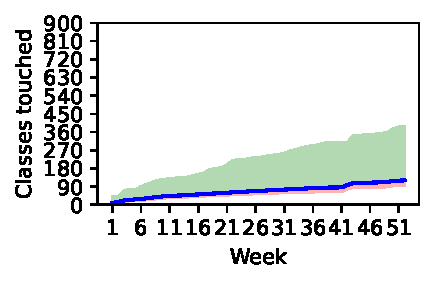
\includegraphics{sections/results/14/classes/time_series_components_touched.classes.all.founders.week_52.pdf}
    \caption{Classes for All founders (n=29, $\mu$=120.68, median=12.0 \& std=142.49)}
    \label{figure.sections/results/14/classes/time_series_components_touched.classes.all.founders.week_52.pdf}
  \end{subfigure}
  \begin{subfigure}[b] 
{0.45\textwidth}
    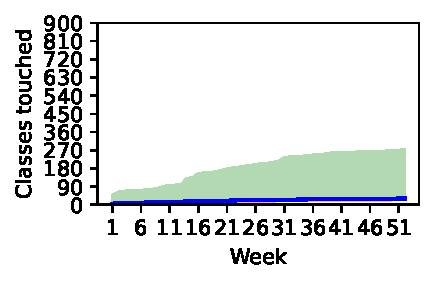
\includegraphics{sections/results/14/classes/time_series_components_touched.classes.all.joiners.week_52.pdf}
    \caption{Classes for All joiners (n=637, $\mu$=31.1, median=3.0 \& std=83.18)}
    \label{figure.sections/results/14/classes/time_series_components_touched.classes.all.joiners.week_52.pdf}
  \end{subfigure}
\newpage 
  \begin{subfigure}[b] 
{0.45\textwidth}
    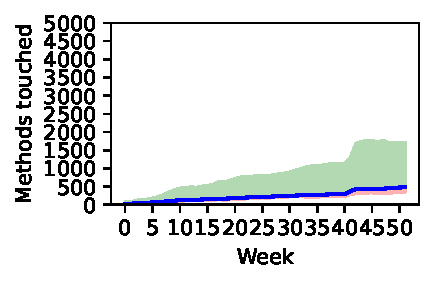
\includegraphics{sections/results/14/methods/time_series_components_touched.methods.all.founders.week_52.pdf}
    \caption{Methods for All founders (n=29, $\mu$=479.85, median=24.0 \& std=576.26)}
    \label{figure.sections/results/14/methods/time_series_components_touched.methods.all.founders.week_52.pdf}
  \end{subfigure}
  \begin{subfigure}[b] 
{0.45\textwidth}
    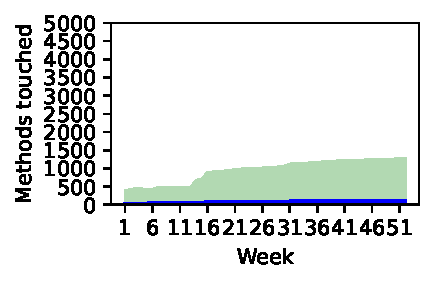
\includegraphics{sections/results/14/methods/time_series_components_touched.methods.all.joiners.week_52.pdf}
    \caption{Methods for All joiners (n=637, $\mu$=110.42, median=7.0 \& std=380.79)}
    \label{figure.sections/results/14/methods/time_series_components_touched.methods.all.joiners.week_52.pdf}
  \end{subfigure}
\caption{Repository 14 A time series for the all commits, excluding transient, with the average mean (blue line), all components touched (y-axis) against the number of week (x-axis) for six (6) developer categories. Green is the standard deviation above the mean, and pink is the standard deviation below the mean.}\end{figure}
\clearpage 
\newpage 
